\chapter{Постановка задачи}
\section{Системы координат}
\noindent\indent В работе используются следующие системы координат:\par
\noindent $OXYZ$ -- невращающаяся система координат: ось $OZ$ направлена
перпендикулярно плоскости эклиптики, $OX$ -- направлена в точку весеннего
равноденствия, а $OY$ дополняет эту систему до правой ортогональной системы
координат, начало координат -- центр масс спутника;\par
\noindent $OX_1X_2X_3$ -- опорная система координат (ОСК). В данной работе
этой системой является орбитальная система координат: ось $OX_1$ направлена вдоль
радиус-вектора, направленного к центру масс спутника от барицентра орбиты его движения
 в поле тяготения Земли, $OX_2$ -- по касательной к траектории орбиты в сторону
движения аппарата, $OX_3$ -- дополняет систему до правой ортонормированной системы
координат, -- направлен перпендикулярно к плоскости орбиты;\par
\noindent $Ox_1x_2x_3$ -- связанная система координат (ССК), оси которой являются
главными центральными осями инерции аппарата.\par
    Связь между системами координат $Ox_1x_2x_3$ и $OX_1X_2X_3$ задается двумя
способами: набором углов $\alpha$, $\beta$, $\gamma$ (рис. \ref{fig:KrilovAngles})
и матрицей направлющих косинусов $A$.\par
    Переход от ОСК к ССК происходит с помощью трех последовательных поворотов
(рис. \ref{fig:KrilovAngles}). Первый поворот осуществляется относительно оси $OX_2$
на угол $\alpha$, второй -- вокруг оси $Ox_3'$ (образованной после первого поворота
осью $OX_3$) на угол $\beta$, третий -- вокруг оси $Ox_1$ на угол $\gamma$.
\begin{figure}[h]
  \centering
  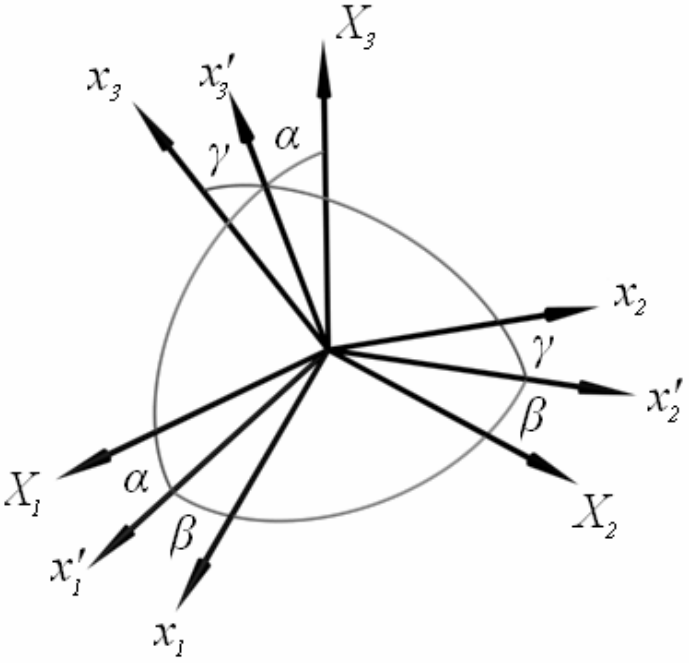
\includegraphics[width=0.4\textwidth]{PlaneAngles}
  \caption{Самолетные углы}
  \label{fig:KrilovAngles}
\end{figure}\par
    Матрица направляющих косинусов через углы Эйлера запишется в виде
\begin{equation}
    A = \begin{bmatrix}
        \cos\alpha\cos\beta & \sin\beta & -\sin\alpha\cos\beta\\
        -\cos\alpha\sin\beta\cos\gamma & \cos\beta\cos\gamma & \sin\alpha\sin\beta\cos\gamma + \cos\alpha\sin\gamma \\
        \cos\alpha\sin\beta\sin\gamma + \sin\alpha\cos\gamma & -\cos\beta\sin\gamma & -\sin\alpha\sin\beta\sin\gamma + \cos\alpha\cos\gamma
    \end{bmatrix}
\end{equation}
Матрица описывает переход из системы координат $OX_1X_2X_3$ в связанную систему
координат $Ox_1x_2x_3$.
\section{Уравнения движения}
\noindent\indent Для описания модели изменения ориентации аппарата, используется
закон изменения кинетического момента (динамические уравнения Эйлера):
\begin{equation}\label{eq:EulerDynamic}
    \dot{\vec{K}} + \vec{\omega}_{\text{абс}} \times \vec{K} = \vec{M}_{\text{вш}} + \vec{M}_{\text{упр}},
\end{equation}
и кинематические уравнения:
\begin{equation}\label{eq:EulerKinematic}
    \dot{A} = WA,
\end{equation}
или
\begin{equation}
    \begin{aligned}
        & \dot{\alpha} = \frac{1}{\cos\beta}(\omega_1\cos\gamma - \omega_3\sin\gamma), \\
        & \dot{\beta} = \omega_2\sin\gamma + \omega_3\cos\gamma, \\
        & \dot{\gamma} = \omega_1 - \tg\beta(\omega_2\cos\gamma - \omega_3\sin\gamma).
    \end{aligned}
\end{equation}
Здесь $\vec{K} = J\vec{\omega}_{\text{абс}}$ -- кинетический момент аппарата;
$\vec{\omega}_{\text{абс}} = \vec{\omega}_{\text{отн}} + A\vec{\omega}_0$ -- вектор
абсолютной угловой скорости; $J$ -- тензор инерции тела; $\vec{M}_{\text{вш}}$ --
момент внешних сил, $\vec{M}_{\text{упр}}$ -- управляющий момент,
$\vec{\omega}_{\text{отн}} = (\vec{\omega}_1\,\, \vec{\omega}_2\,\, \vec{\omega}_3)^T$ --
вектор угловой скорости движения системы $Ox_1x_2x_3$ относительно $OX_1X_2X_3$,
записанный в осях системы $Ox_1x_2x_3$, $\vec{\omega}_0$ -- абсолютная угловая
скорость системы координат $OX_1X_2X_3$, матрица $W$ имеет вид
\begin{equation}
    W = \begin{bmatrix}
        0 & \omega_3 & -\omega_2 \\
        -\omega_3 & 0 & \omega_1 \\
        \omega_2 & -\omega_1 & 0
    \end{bmatrix}.
\end{equation}
\noindent\indent Система уравнений, описывающих движение тела по орбите
под действием возмущающих ускорений выглядит следующим образом:
\begin{equation}
  \begin{cases}
    \frac{dp}{dt} = 2r\sqrt{\frac{p}{\mu}}T, \\
    \frac{de}{dt} = \sqrt{\frac{p}{\mu}}\left\{
      S\sin\nu + T\left[(1 + \frac{r}{p})\cos\nu + e\frac{r}{p}\right]
    \right\}, \\
    \frac{d\omega}{dt} = \frac{1}{e}\sqrt{\frac{p}{\mu}}\left[
      -S\cos\nu + T(1 + \frac{r}{p})\sin\nu - W e\frac{r}{p}\sin u\ctg i
    \right] \\
    \frac{di}{dt} = W \frac{r}{\sqrt{\mu p}}\cos u, \\
    \frac{d\Omega}{dt} = W \frac{r}{\sqrt{\mu p}}\frac{\sin u}{\sin i}, \\
    \frac{d\tau^*}{dt} = \frac{r^2}{e\mu}\left[
      S (eN\sin\nu - \cos\nu) + T N\frac{p}{r}
    \right],
  \end{cases}
\end{equation}
где
\begin{equation}
  N = \frac{p^2}{r^2}\int\limits_0^{\nu} \frac{2\cos\nu}{(1 + e\cos\nu)^3}d\nu,\,\,
  u = \nu + \omega.
\end{equation}
Здесь $p$ -- параметр орбиты, $e$ -- эксцентриситет орбиты, $\omega$ -- аргумент
перигея, $i$ -- наклонение, $\Omega$ -- долгота восходящего узла, $u$ -- аргумент
широты, $\tau^*$ -- параметр положения объекта на орбите в каждый момент времени,
$S$, $T$, $W$ -- соответственно радиальное, трансверсальное и нормальное возмущающие
ускорения.
Начальные условия задаются следующим образом:
\begin{equation}
\begin{aligned}
    & p(t_0) = p_0, \\
    & e(t_0) = e_0,\,\, e_0 \in (0, 1), \\
    & \omega(t_0) = \omega_0, \\
    & i(t_0) = i_0, \\
    & \Omega(t_0) = \Omega_0, \\
    & \tau^*(t_0) = \tau^*_0
\end{aligned}
\end{equation}\par
    Элементарная сила светового давления, возникающего под действием солнечного излучения записывается
следующим образом:
\begin{equation}
  d\vec{F}_{\text{SRP}} = P(R) \cdot \left[
    -a_{10}(\vec{n}\cdot\vec{s})\vec{s}
    +a_{20}(\vec{n}\cdot\vec{s})\vec{n}
    -2a_{30}(\vec{n}\cdot\vec{s})^2\vec{n}
  \right]dA,
\end{equation}
здесь
\begin{equation}
  P(R) = \frac{q_0(R)}{c},
\end{equation}
-- световое давление ($q_0(R)$ -- солнечная постоянная, которая зависит от
расстояния $R$ до Солнца, $c$ -- скорость света в вакууме); $a_{10}$, $a_{20}$,
$a_{30}$ -- обобщенные оптические параметры, определяемые следующим образом:
\begin{equation}
  \begin{aligned}
    & a_{10} = 1 - \rho s, \\
    & a_{20} = B_f\rho(1 - s) + (1 - \rho)\frac{\epsilon_f B_f - \epsilon_b B_b}{\epsilon_f + \epsilon_b}, \\
    & a_{30} = \rho s, \\
  \end{aligned}
\end{equation}
причем $\rho$ -- коэффициент зеркального отражения; $s$ -- коэффициент зеркальности;
$B_f$ и $B_b$ -- коэффициенты, показывающие характер индикатрисы отражения за вычетом
зеркальной составляющей (в случае диффузного отражения $B = 2/3$); $e_f$ и $e_b$ --
излучательная способность освещенной и обратной стороны паруса.\par
  Параметры $a_{10}$ и $a_{30}$ учитывают зеркальную составляющую, а первое слагаемое
параметра $a_{20}$ в случае, когда $B_f$ и $B_b = 2/3$, -- диффузную составляющую.
Второе слагаемое параметра $a_{20}$ отвечает за вклад собственного теплового излучения
полотна в результирующую силу светового давления.\par
  Аналогично запишем выражения для момента от элементарной силы светового давления
\begin{equation}
  d\vec{M}_{\text{SRP}} = \vec{r} \times d\vec{F} = P(R) \cdot \left[
    -a_{10}(\vec{n}\cdot\vec{s})(\vec{r} \times \vec{s})
    +a_{20}(\vec{n}\cdot\vec{s})(\vec{r} \times \vec{n})
    -2a_{30}(\vec{n}\cdot\vec{s})^2(\vec{r} \times \vec{n})
  \right]dA,
\end{equation}
где $\vec{r}$ -- вектор, задающий положение элементарной площадки $dA$.\par
  Векторы $\vec{s}$ и $\vec{n}$ задаются в ОСК выражениями\par
\begin{equation} \label{eq:SunVector}
  \vec{s} = \begin{bmatrix}
     \sin\psi_s\sin\theta_s \\
    -\cos\psi_s\sin\theta_s \\
     \cos\theta_s
  \end{bmatrix},
\end{equation}
\begin{equation}
  \vec{n} = \begin{bmatrix}
     \sin\psi\sin\theta \\
    -\cos\psi\sin\theta \\
     \cos\theta
  \end{bmatrix}.
\end{equation}\par
Связь компонент вектора Солнца $\vec{s}$ с положением плоскости орбиты относительно
направления на Солнце выявляется из сравнения (\ref{eq:SunVector}) и альтернативного
выражения
\begin{equation}
  \vec{s} = \begin{bmatrix}
    \sigma_x\cos u + \sigma_y\sin u \\
    \sigma_y\cos u - \sigma_x\sin u \\
    \sigma_z
  \end{bmatrix}
\end{equation}
через компоненты вектора $\sigma$, связанные с долготой восходящего узла $\Omega$,
наклонением $i$ и эклиптической долготой $\lambda$ по формулам
\begin{equation}
\begin{aligned}
    & \sigma_x =  \cos\Omega\cos\lambda + \sin\Omega\sin\lambda\cos\epsilon, \\
    & \sigma_y =  \cos\Omega\cos i\sin\lambda\cos\epsilon - \sin\Omega\cos i\cos\lambda + \sin i\sin\lambda\sin\epsilon, \\
    & \sigma_z = -\cos\Omega\sin i\sin\lambda\cos\epsilon + \sin\Omega\sin i\cos\lambda + \cos i\sin\lambda\sin\epsilon,
\end{aligned}
\end{equation}
где $\epsilon = 23^o26'$ -- наклон эклиптики к экватору. Имеем:
\begin{equation}
  \begin{aligned}
    & \theta_s = \arccos\sigma_z, \\
    & \psi_s = atan2(\sigma_x\cos u + \sigma_y\sin u, \sigma_x\sin u - \sigma_y\cos u).
  \end{aligned}
\end{equation}
Функция $atan2$ обозначает операцию взятия обратного тангенса с учетом знаков
обоих аргументов.\par
    Для учета нахождения космического аппарата в области тени и полутени вводят,
так называемую, <<функцию тени>>, что представляет из себя скалярную функцию, зависящую
от положения спутника относительно Земли и Солнца. В виду сложности эффекта
отбрасывания тени Землей и нечеткости границы полутени, в качетсве функции тени
часто берется не <<релейная>>, непрерывная, функция, аппроксимирующую реальные
свойства тени, типа функции, изображенной на (рис. \ref{fig:shadowFunction}).
\begin{figure}[h!]
  \centering
  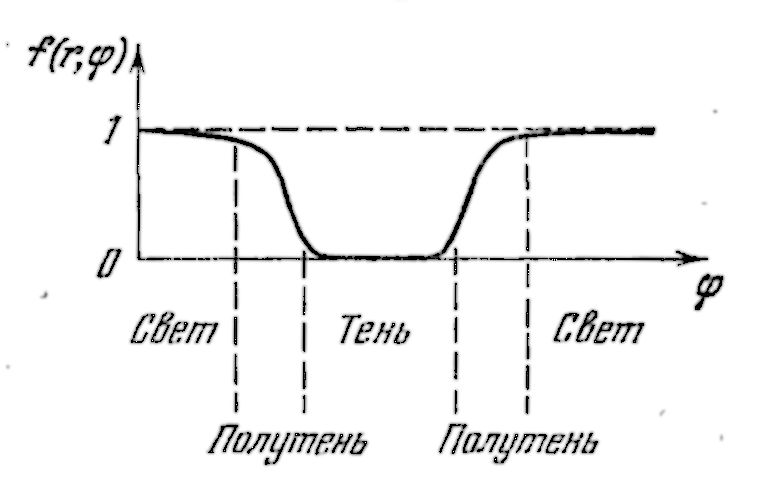
\includegraphics[width=0.6\textwidth]{shadowFunction}
  \caption{Функция тени}
  \label{fig:shadowFunction}
\end{figure}
Где $r$ -- вектор, направленный от центра Земли к центру масс спутника; $\phi$
-- угол между вектором, направленным вдоль вектора, пущеного из центра Солнца к
центру Земли и вектором $r$.\par
    Одни из наиболее влияющих на движение низкоорбитальных спутников (т.е. спутников,
движущихся на высотах от 150 до 1500 км) сил негравитационной природы оказываются
аэродинамические силы, вызванные влиянием атмосферы Земли.\par
    Сила, действующая на парус, при сопротивлении атмосферы, записывается в
следующем виде:
\begin{equation}
    \vec{F}_{\text{a}} = -\frac{C_d A}{2}\rho|\vec{v}_{\text{отн}} \cdot \vec{n}| \vec{v}_{\text{отн}},
\end{equation}
где $C_d$ -- коэффициент лобового сопротивления (принимаем равным стандартному
значению $2.2$), $\rho$ -- плотность атмосферы, $\vec{v}_{\text{отн}}$ --
скорость КА с парусом относительно набегающего потока. Для простоты рассчитываем
посленее в приближении плотностью увлекаемой Землей атмосферы
\begin{equation}
    \vec{v}_{\text{отн}} = \vec{v} - \vec{\omega}_{\oplus} \times \vec{r} =
\sqrt\frac{\mu}{p}\begin{bmatrix}
           e_x\sin u - e_y\cos u \\
           1 + e_x\cos u + e_y\sin u \\
           0
         \end{bmatrix} - \omega_{\oplus}r\begin{bmatrix}
                    0 \\
                    \cos i \\
                    \sin i \cos u
                  \end{bmatrix},
\end{equation}
где $\omega_{\oplus} \approx 7.29\cdot 10^{-5} \text{с}^{-1}$ -- скорость вращения
Земли вокруг своей оси.\par
    Также запишем выражения для аэродинамического момента:
\begin{equation}
    \vec{M}_{\text{a}} = \frac{C_d A}{2}\rho|\vec{v}_{\text{отн}} \cdot \vec{n}| \vec{v}_{\text{отн}}\times\vec{r}
\end{equation}
